Next a slice at $z=\SI{40}{nm}$ is compared to the original simulation by \cite{heeg} in figure \ref{fig:slice-comparision}. The overal local enhancement of the simulation reproduces the original simulation. The biggest difference is noticeable right at the outer edges of the nanostructure: Compared to the original simulation the enhancement is slightly bigger.

\begin{figure}[!h]
  \centering
  \begin{subfigure}{0.50\textwidth}
    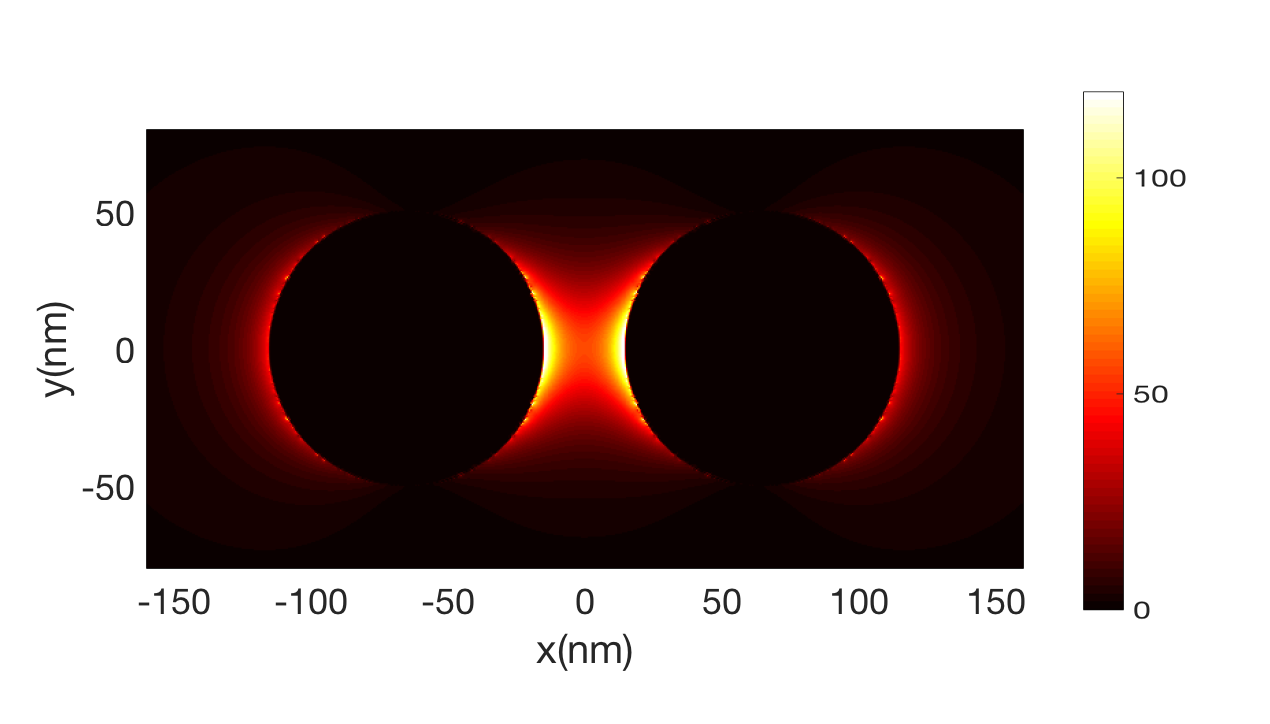
\includegraphics[width=\textwidth]{./images/40nm.png}
  \end{subfigure}
  ~
  \begin{subfigure}{0.40\textwidth}
    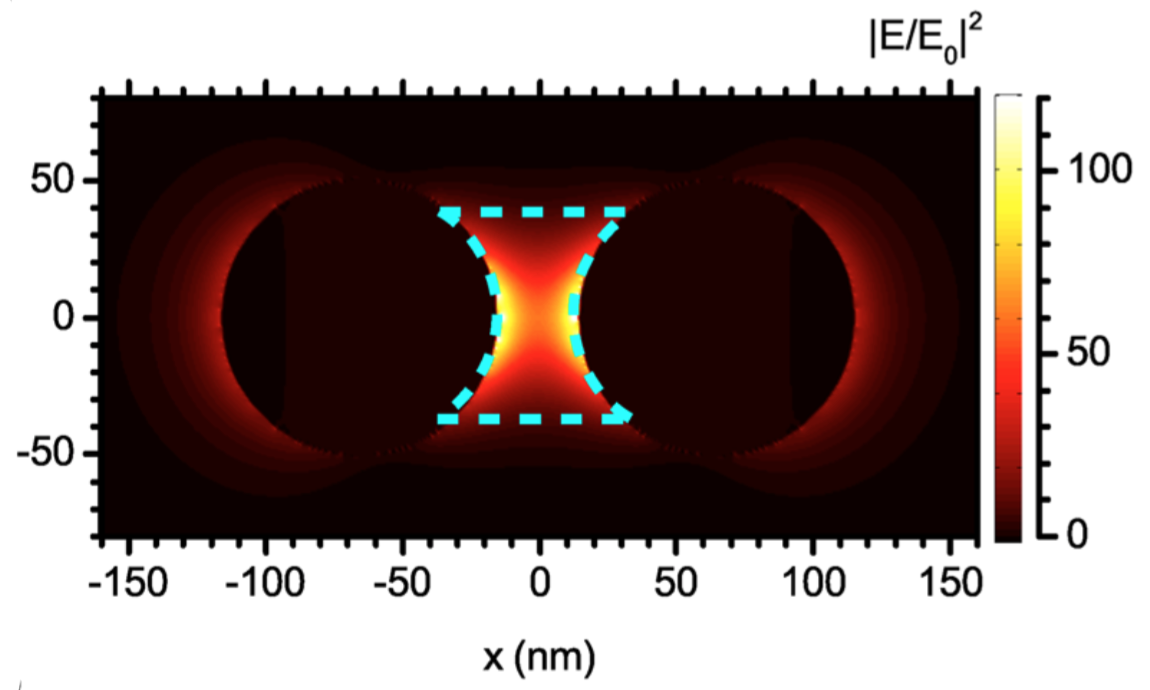
\includegraphics[width=\textwidth]{./images/local-enhancement-heeg.png}
  \end{subfigure}
  \caption{\textbf{(a)} Near field enhancement $|E/E_0|^2$ in the $x,y$-plane at $z=\SI{40}{nm}$. \textbf{(b)} Original results by \cite{heeg}.}
  \label{fig:slice-comparision}
\end{figure}

This difference is also noticeable by plotting a the near field enhancement in the $x,z$ plane at $y=0$ in figure \ref{fig:yline}.

\begin{figure}[!h]
  \centering
  \begin{subfigure}{0.45\textwidth}
    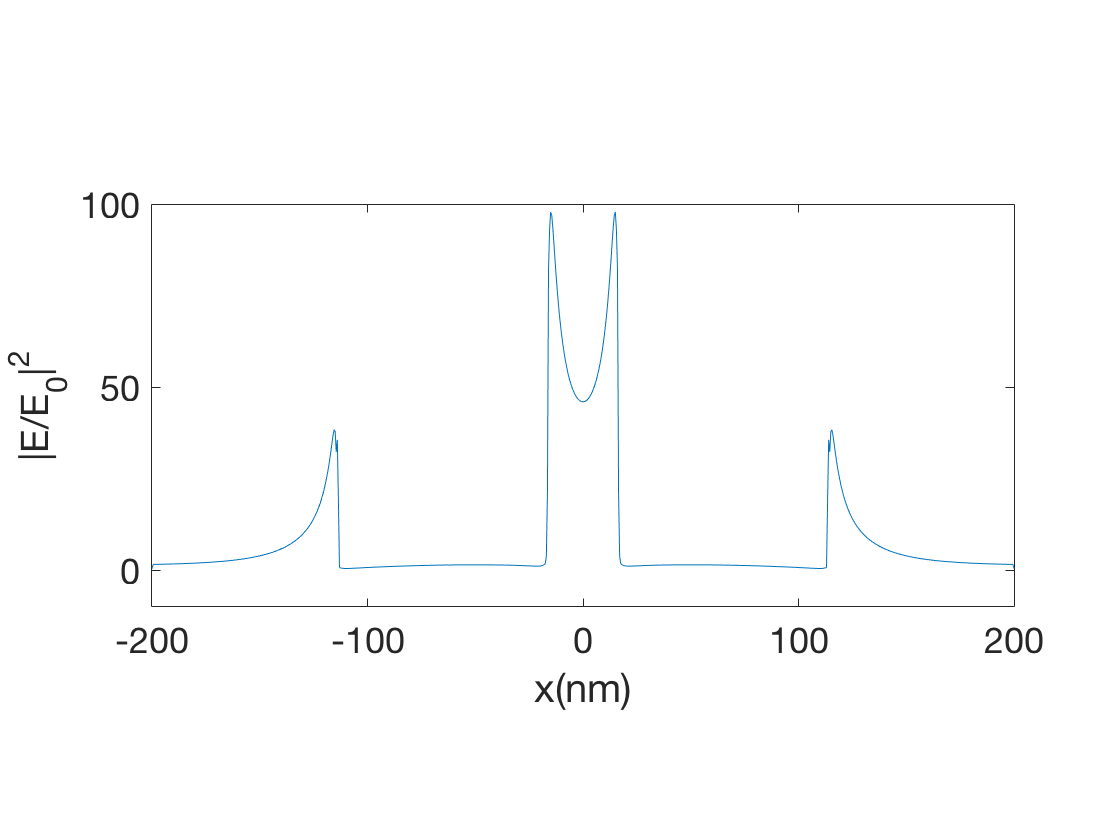
\includegraphics[width=\textwidth]{./images/40nm-y.png}
  \end{subfigure}
  ~
  \begin{subfigure}{0.45\textwidth}
    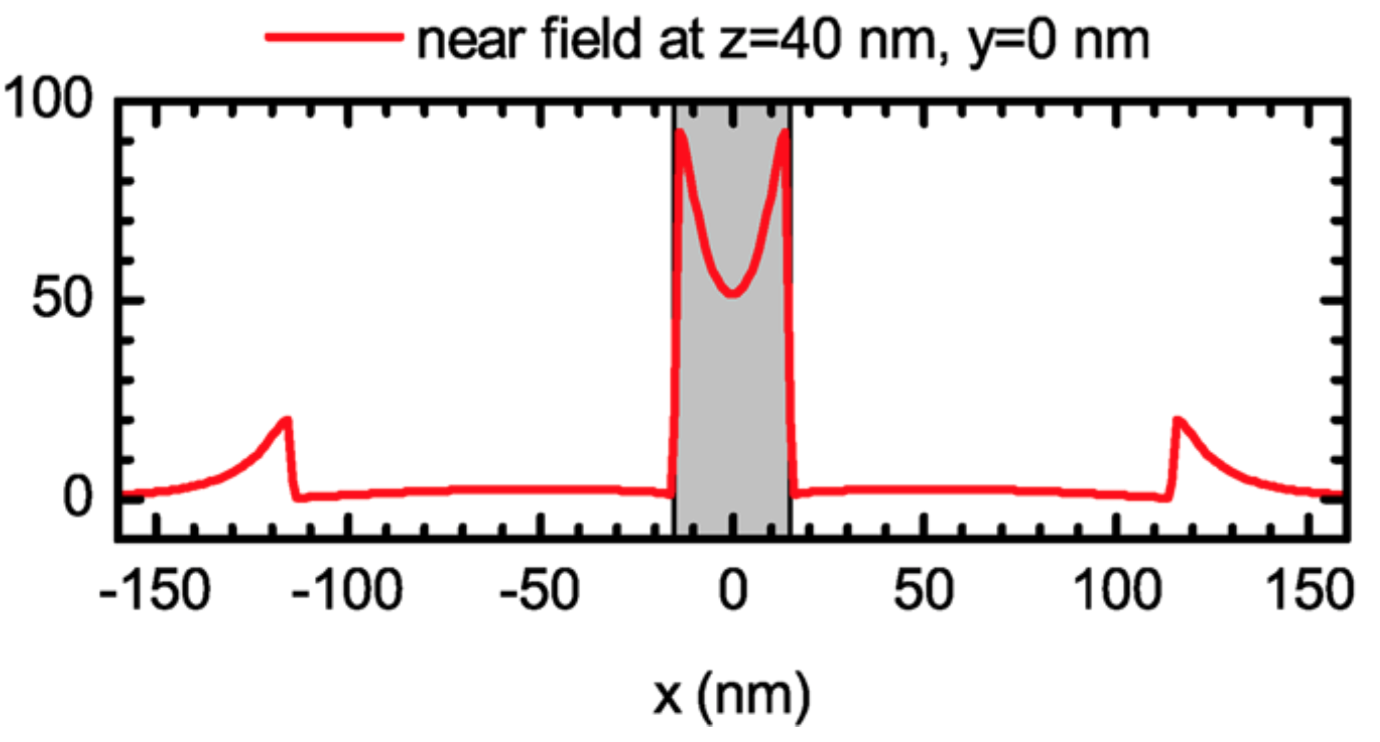
\includegraphics[width=\textwidth]{./images/heeg-y-line.png}
  \end{subfigure}
  \caption{\textbf{(a)} Near field enhancement $|E/E_0|^2$ in the $x,z$-plane at $y=0$. \textbf{(b)} Original results by \cite{heeg}.}
  \label{fig:yline}
\end{figure}

The graph has approximately the same shape and values within the cavity, with a maximum enhancement of $100$ at the edges of the cavity and a minimum enhancement of $50$ within the cavity. The biggest difference again is visible at the outer edges of the gold nanostructure.

These differences can be explained with the different corner radiuses where sharper edges lead to a higher enhancement. But because the outer enhancement can neglected compared to the enhancement within the cavity according to \cite{heeg} the results of the simulation will be assumed as matching the original paper's simulation.
